\documentclass[11pt,a4paper,sans]{moderncv}
\usepackage{graphicx}

% CV style and color configuration
\moderncvstyle[nosymbols]{banking}
\moderncvicons{awesome}
\moderncvicons{tikz}
\DeclareFontSeriesDefault[sf]{bf}{bx}
\moderncvcolor{blue}
\colorlet{firstnamecolor}{black}
\colorlet{lastnamecolor}{black}
\renewcommand*{\labelitemi}{\strut\textcolor{black}{\small\rmfamily\textbullet}}

% Set margins to fit one page
\usepackage[scale=0.82]{geometry}  

% Personal information
\name{Thinh Nguyen Nhu}{}
\address{Hanoi University of Science and Technology, Hanoi, Vietnam}{}{}
\email{nhuthinh2004@gmail.com}
\phone{0329 000 482}
\providecommand{\orcid}[1]{\def\@orcid{#1}}
\orcid{0009-0002-8653-2368}
\begin{document}

\makeatletter
\noindent
\begin{minipage}[c]{0.78\textwidth}
    \raggedright
    \firstnamestyle{\@firstname}~\lastnamestyle{\@lastname}\par
    \vspace{0.5em}
    \addressstyle{\@addressstreet}\par
    \vspace{0.3em}
    \addressstyle{\emailsymbol\emaillink{\@email}\quad
    \collectionloop{phones}{\csname\collectionloopkey phonesymbol\endcsname\collectionloopitem}%
    \@ifundefined{@orcid}{}{\quad\href{https://orcid.org/\@orcid}{ORCID: \@orcid}}}\par
\end{minipage}\hfill
\begin{minipage}[c]{0.18\textwidth}
    \raggedleft
    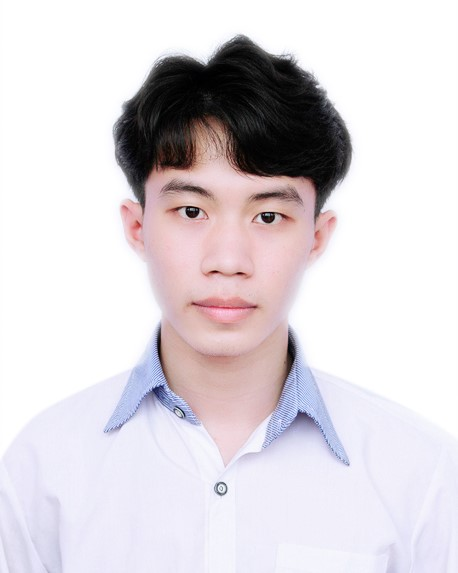
\includegraphics[width=\linewidth]{thinh.jpg}
\end{minipage}
\makeatother
\par\vspace{1em}

\section{Introduction}
As a science-oriented person, my long-term vision is to develop intelligent systems and structures that learn from the fundamental principles of physics, biology, and engineering. My research interests focus on applied machine learning, particularly Physics-Informed Machine Learning (PIML) and Generative AI for scientific discovery and inverse problems. My ultimate goal is to build physics-grounded AI models that enable the understanding, design, and control of next-generation smart systems.

\section{Education}
\cventry{11/2026 -- Present}
        {M.Sc. in Mechatronics Engineering}
        {Hanoi University of Science and Technology (HUST)}
        {\textnormal{Hanoi, Vietnam}}
        {}{}

\cventry{10/2022 -- 08/2026}
        {B.Sc. in Mechatronics Engineering}
        {Hanoi University of Science and Technology (HUST)}
        {\textnormal{Hanoi, Vietnam}}
        {}{}
\cvitem{\textnormal{GPA}}{3.69 / 4.0}
\cvitem{\textnormal{Thesis}}{Modeling and Inverse Design of Kresling Origami via Physics-Informed Neural Networks}

\section{Research \& Projects}

\cventry{09/2026 -- Present}
        {Research Assistant}
        {AiRA Lab (\href{https://aira-hust.github.io/AiRA/}{AiRA}), HUST}
        {\textnormal{Hanoi, Vietnam}}
        {}
        {\begin{itemize}
        \item Investigate Physics-Informed Machine Learning (PIML) methods for scientific and engineering applications.
        \item Develop PINN architectures for multi-solution inverse design of Kresling Origami structures.
        \item Conduct molecular dynamics (MD) simulations and structural design of DNA Origami; explore AI-driven approaches for DNA Origami property prediction and design.
        \item Serve as Teaching Assistant for the course \href{https://github.com/AiRA-Laboratory/AI4SE}{AI for Science and Engineering (AI4SE)}.
        \end{itemize}}

\cventry{12/2025 -- Present}
        {Research Collaborator}
        {\begin{tabular}[t]{@{}l@{}}ICMAM Lab Collaborative\\Ho Chi Minh City University of Technology (HCMUT)\end{tabular}}
        {\textnormal{Ho Chi Minh City, Vietnam}}
        {}
        {\begin{itemize}
        \item Apply Physics-Informed Neural Networks (PINN) for structural analysis and design optimization of composite laminates based on First-order Shear Deformation Theory (FSDT).
        \end{itemize}}

\cventry{07/2025 -- Present}
        {Research Student}
        {Origami Technology Lab, HUST}
        {\textnormal{Hanoi, Vietnam}}
        {}
        {\begin{itemize}
        \item Modeled nonlinear dynamic behaviors of Kresling origami and constructed bifurcation diagrams under harmonic excitation.
        \item Formulated Physics-Informed Neural Network (PINN) algorithms for the inverse design of Kresling structures as part of undergraduate thesis research.
        \item Perform numerical dynamic modeling of Magnetically Actuated Kresling Origami combining magnetic actuation with a bar-and-hinge framework and the open-source Newton-Physics environment.
        \end{itemize}}

\cventry{10/2024 -- 06/2025}
        {Undergraduate Student}
        {Project XYaZ Lab, HUST}
        {\textnormal{Hanoi, Vietnam}}
        {}
        {\begin{itemize}
        \item Modeled and simulated the dynamics of a 3-RRR planar parallel robot using MATLAB/Simulink.
        \item Evaluated trajectory-tracking algorithms for parallel mechanisms.
        \end{itemize}}

\section{Publications}

\cvitem{}{\textbf{Spatial Dynamic Modeling of Magnetically Actuated Kresling Origami: A Bar-and-Hinge Framework}, \underline{Thinh Nguyen Nhu}, Duy Pham Minh, Chien Truong-Quoc\textsuperscript{*}, Thao Thai Phuong\textsuperscript{*}; \textit{ICOMMA 2027 (in preparation)}, 2026.}

\cvitem{}{\textbf{Gradient-Based Inverse Design of Kresling Origami via Neural Surrogate Modeling}, Thanh Trung Vuong, Duc Thu Nguyen, \underline{Nguyen Nhu Thinh}, Thao Thai Phuong*, Chien Truong Quoc*; \textit{Robotics and Mechatronics, ISRM 2026}; 03 Jul 2026, [\href{https://doi.org/10.1007/978-3-032-29469-2_39}{10.1007/978-3-032-29469-2\_39}].}

\cvitem{}{\textbf{A Comprehensive Analysis of Global Dynamics and Bifurcation of a Kresling Origami Structure}, Minh-Tuan Nguyen-Thai; \underline{Thinh Nguyen Nhu}; Ngoc-Vu Le-Nguyen; Chien Truong-Quoc*; Thao Phuong Thai*; \textit{submitted}; 2026, [\href{https://doi.org/10.2139/ssrn.6721329}{10.2139/ssrn.6721329}].}

\cvitem{}{\textbf{Dynamic Behavior of Kresling Origami under Harmonic Excitation: A Five-Parameter Energy Framework}, \underline{Thinh Nguyen Nhu}, Chien Truong Quoc*, Thao Thai Phuong*; \textit{The 8th International Conference on Engineering Mechanics and Automation (ICEMA25)}; 14 Nov 2025, [\href{https://doi.org/10.15625/vap.2026.0031}{10.15625/vap.2026.0031}].}

\section{Skills}
\cvitem{Programming}{Python, PyTorch, JAX, MATLAB/Simulink, C/C++}
\cvitem{Machine Learning}{Physics-Informed Machine Learning (PIML), Operator Learning, Kolmogorov–Arnold Networks (KAN), Generative Modeling (VAE, Diffusion), CNN}
\cvitem{Molecular Dynamics}{Molecular Dynamics (MD) Simulation, cadnano, tacoxDNA, oxDNA}
\cvitem{Mathematical Tools}{Optimization, Mathematical modeling of dynamical systems, Numerical simulation, Newton-Physics open-source simulation engine, Nonlinear system analysis, FEA}
\cvitem{Misc.}{Academic research, Reading scientific literature and writing in English, LaTeX typesetting, research presentations}

\section{Achievements}
\cvitem{}{\textbf{Certificate of Merit for Outstanding Graduate} -- Hanoi University of Science and Technology (awarded for university-wide outstanding graduation: CPA \textgreater{} 3.6 and Training Score \textgreater{} 90). (09/2026)}
\cvitem{}{\textbf{Academic Encouragement Scholarship} for semesters 2023.2, 2024.1, 2024.2, and 2025.2 -- HUST.}
\cvitem{}{\textbf{Outstanding Creative Idea Award} - 43rd HUST Annual Student Research Conference (SVNCKH), HUST. (2026)}
\cvitem{}{\textbf{VPMS Award} - Graduation Thesis with Scientific Value, HUST. (2026)}
\cvitem{}{\textbf{Certificate of Merit for Outstanding Student}, Academic Year 2024--2025, HUST. (2025)}

\section{References}
\cventry{School of Mechanical Engineering, HUST}
        {thao.thaiphuong@hust.edu.vn}
        {Thao Thai Phuong, PhD}
        {\textnormal{Lecturer}}
        {}{}
\cventry{School of Mechanical Engineering, HUST}
        {chien.truongquoc@hust.edu.vn}
        {Chien Truong-Quoc, PhD}
        {\textnormal{Lecturer}}
        {}{}

\end{document}